
\section{Overview}

A diagram showing the overall system design can be seen in Figure \ref{fig:SystemDesign}. The components of this diagram will be further explained below.

\begin{figure}[h]
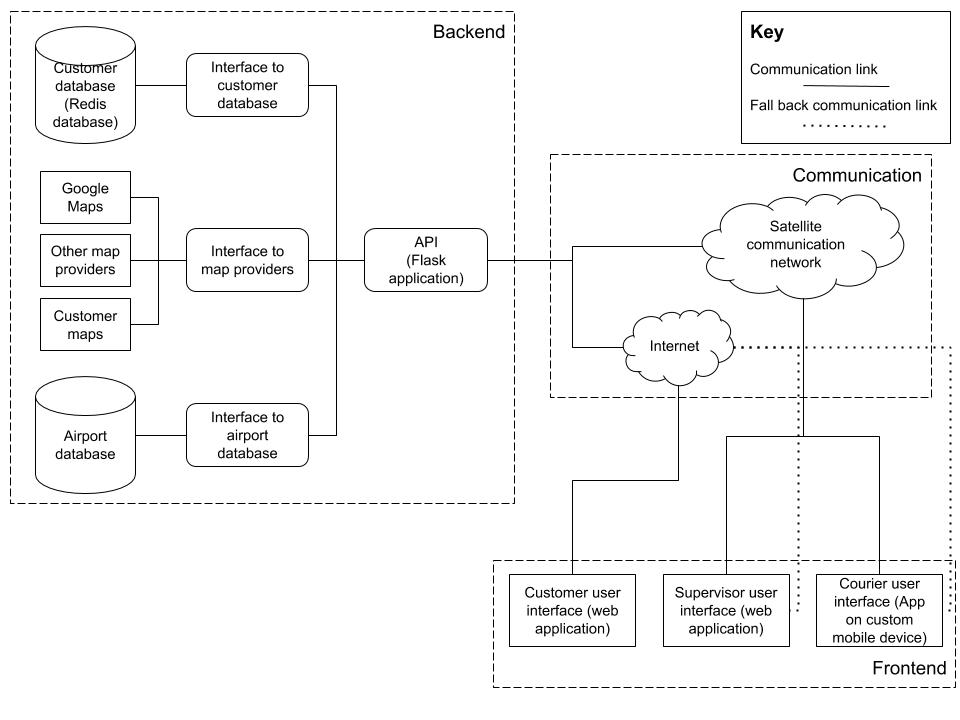
\includegraphics[scale=0.5]{SystemDesign.jpg}
    \centering
    \caption{Diagram of the overall system design}
    \label{fig:SystemDesign}
\end{figure}

\section{Front-end} \label{frontendarch}
In order to allow the users to interact with our system, we have designed an interface for each user type. We can distinguish three different types of people that will need to access and alter the appropriate elements of our product. First, there are the couriers which must be given instructions to follow together with the recipient information such as constraints. Next, we have the supervisors which are responsible for guiding the couriers and passing optimal routes to them. Finally we have the customers of our system that should be notified about the progress of their delivery.

Each user will have their own login and password with which they can access their account on the appropriate application. To ensure that the data passed between the supervisors and couriers is secure, it will be sent through our own network described in Section \ref{networkarch}. The information shared with the customer accounts will be limited, therefore in the design we propose to pass encrypted messages through ordinary internet connection available to everyone. This also takes the pressure off the satellite network.

\subsection{Supervisor application} \label{supervisorsarch}
The most complex front end component is the application for the supervisors, which will be used in the control room. It will be implemented as a dynamic web application. Once a supervisor logs in to the system, they will be able to open the following views available through the navigation bar at the top of the page:
\begin{itemize}
    \item Map - this view will present a world map with current locations of all couriers and briefcases which are currently on a delivery mission. In case of an emergency, the courier marker will flash red. This will be useful to inspect progress of each courier and quickly understand the concept of possible threats if a courier is marked in red.
    \item Couriers - allows the supervisors to create new courier accounts in the database and edit the existing ones. They will be able to see the details of each courier including their current location and status. Another key feature of this view enables communication with each courier by sending/receiving direct text messages.
    \item Customers - simple view allowing for creation and edition of customer records. The supervisor will also be able to see any previous orders from each customer. The supervisor will also be able to add constraints that relate to all deliveries for a certain customer.
    \item Deliveries - allows for creation and edition of delivery missions. During the creation process, a supervisor will be able to select the sender and recipient from of the delivery, allocate multiple couriers to a mission and add any constraints to the route. Once all of those options have been selected, a route will be generated. The supervisor can then inspect the route and correct it by adding points to go through if necessary before adding the delivery to the database.
    \item Server logs - allows for inspection of every modification made to the database. The server logs will be created after each request updating the database and no one will be able to change them in any way. In case of a human error the contents of server logs will be a clear proof of who is responsible for it. 
\end{itemize}
\subsection{Courier application} \label{couriersarch}
Since the couriers will be moving around the globe, the best way for them to interact with the system will be through a smart phone device. Each courier will be provided with a phone with our mobile courier application installed on it, which can only connect with our satellites. 

The app will allow a registered courier to see the route for the delivery that he/she is currently assigned to, together with a schedule and a set of step by step instructions containing additional information about any hotels/tickets booked by the control room. They will also be provided with the recipient's contact details. The courier will also be able to communicate with the control room with use of text messages through the application in case of additional questions or reporting a problem. 

The device will send the couriers position in short intervals to allow the control room to track their location in real time.

\subsection{Customer application} \label{customersarch}
To promote our services to our potential customers we will create a website which describes them clearly. The website will allow the user to register as a customer and order deliveries by giving the details of a sender and recipient together with a deadline. A customer will then be able to see crucial events about their deliveries together with an ETA of delivery.


\section{Back-end} \label{backendarch}
\subsection{Customer database} \label{databasearch}
The first component of the backend is a database of customer and staff information. Its most important task is storing delivery information and constraints, which are merged with the maps database to provide directions to the courier. It is designed to store the following datatypes:

\begin{itemize}
    \item Customer
    \item Delivery
    \item Constraint (delivery deadline, allowed transport methods, and areas to avoid)
    \item Courier
    \item Supervisor
    \item Message (messages between supervisors and couriers)
    \item DeliveryEvent (significant delivery events, such as "picked up by courier" or "delivered", used to keep an audit trail for each delivery)
\end{itemize}

Full details of the structure of each data type can be found in Appendix \ref{databaseAppendix}. The most complex type is the constraint. These exist on three levels: delivery, customer, and overall. Every delivery has its own constraints, allowing specific objects to be transported according to particular requirements. Every customer can have constraints applied to all of the deliveries where they are the sender. For example, government bodies may wish for none of their packages to cross countries they have strained diplomatic relations with. Finally, overall constraints are applied to all deliveries. These are applied when it becomes unsafe for anyone to traverse a particular area. Additional to these constraints we store staff contact and authentication data.

\begin{figure}[h]
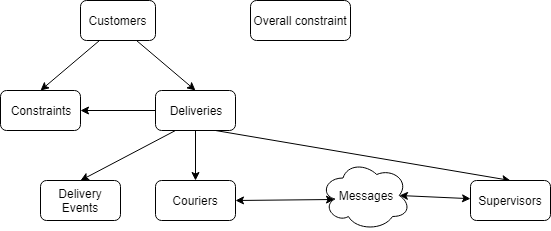
\includegraphics[scale=0.5]{database_outline.png}
    \centering
    \caption{Outline of Redis database}
    \label{fig:redis_database}
\end{figure}

This information will be stored in a Redis database within a Docker container, for ease of setup and added security. Redis was chosen for its efficiency and security - it is a simple database designed with speed in mind, and has measures in place to avoid third party attacks\cite{redisSecutiry}. It allows us to rename and disable commands such that potential attackers cannot send commands to the database. We will use this to ban clearing the database contents, and obscure all commands used by the API code. Redis has no concept of string escaping, making injection attacks impossible. It does not support encryption, but to compensate for this we will use a firewall to block all but the API server from communicating with it, and encrypt all API responses.

A set of Python functions will be defined to verify and process data sent to Redis such that it contains the attributes and data types described. These functions are to be used by a class called RedisInterface. This is a wrapper around the Redis Python package, implementing functions for adding and retrieving all of the above objects.

An API layer will be written on top of this using Flask, allowing the frontend to access, update, and delete data without needing knowledge of which RedisInterface methods to call. This API will also be enclosed in a Docker container, allowing us full control of the API server. The architecture of the Redis API is summarised in the following figure.

\begin{figure}[h]
    \centering
    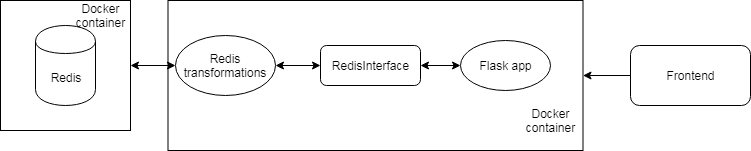
\includegraphics[scale=0.5]{redis_backend_diagram.png}
    \caption{Redis API software architecture}
    \label{fig:redis_architecturel}
\end{figure}

The API is designed with the database structure in mind, providing simple links to constraints on all levels, lists of staff and customers, as well as specific information retrievable by ID. The following table provides a list of URLs, callable methods, and expected API responses.

\begin{center}
\begin{tabular}{ | m{6.1cm} | m{3.8cm}| m{6cm} | } 
\hline
URL & Methods & Description \\
\hline
/constraints/overall & GET, POST, DELETE & Get, modify, or remove overall constraints \\
\hline
/constraints/customer/<customerId> & GET, POST, DELETE & Get, modify, or remove a specific customer's constraints \\
\hline
/constraints/delivery/<deliveryId> & GET, POST, DELETE & Get, modify, or remove a specific delivery's constraints\\
\hline
/customers & GET, POST & Get the full list of customers, or add a customer\\
\hline
/customers/<customerId> & GET, PUT, DELETE & Get, update, or remove a customer's data\\
\hline
/couriers & GET, POST & Get the full list of couriers, or add a courier\\
\hline
/couriers/<courierId> & GET, PUT, DELETE & Get, update, or remove a courier's data\\
\hline
/supervisors & GET, POST & Get the full list of supervisors, or add a supervisor\\
\hline
/supervisors/<supervisorId> & GET, PUT, DELETE & Get, update, or remove a supervisor's data\\
\hline
/deliveries & GET, POST & Get the full list of deliveries, or add a delivery\\
\hline
/deliveries/<deliveryId> & GET, PUT, DELETE & Get, update, or remove a delivery\\
\hline
/deliveries/customer/<customerId> & GET & Get all deliveries where a particular customer is either sender or receiver\\
\hline
/events/<deliveryId> & GET & Get all of a delivery's events\\
\hline
/messages & GET, POST & Get all messages sent or received by a specific person, or add a message\\
\hline
\end{tabular}
\end{center}

\subsection{Maps API} \label{mapsarch}

The second major component of the backend part of the system is the mapping and routing API which is used by the couriers to get step by step directions and by supervisors to view and confirm the routes that couriers will take.

As with the database API this is a RESTful API that provides responses in JSON and runs as part of a flask app. The whole API (both the database API and the routing API) are part of the same flask app that can easily be called by the frontend part of the system.

The system will primarily rely on Google Maps \cite{GoogleMaps} for its mapping data however along with this customers will be able to provide their own mapping data. For example a customer may have a more detailed map of a certain area that can be used along side the data from Google Maps to provide better routing. We are also planning to expand to a wider range of commercial mapping providers after the system is launched so we are no longer relying on a single one. When using these commercial mapping providers we will send some fake requests to their APIs along with the real ones in an effort to hide the location of our couriers from third parties.

Along with providing maps, customers will also be able to provide constraints that apply to the routes their packages take when being delivered. These can be specified for all deliveries or just for individual packages depending on the customers needs. For example a customer may not wish for their packages to travel through countries where they have no diplomatic relations as this may leave them vulnerable.

\section{Communication} \label{communicationarch}
Communication between the front-end and back-end components can take place through one of two channels at any time. The primary channel is our private satellite network, this will be used whenever possible and it is hoped to be the only method of communication once the full network is operational. The backup communication channel is the internet, this will be used only when the satellite network is unavailable as it is less secure and only with the customers approval. 

All transmissions through both channels will be end-to-end encrypted to protect their contents. The method of encryption used may vary based on the requirements of the customer. In order to further obfuscate our communications, each real transmission will be accompanied by a random number of fake transmissions. This will make finding our real communications significantly harder.

\subsection{Private Satellite Network} \label{networkarch}
A private satellite network will be launched. Initially, this network will only cover a small area of the globe (this area will likely be decided through feedback from potential customers). Revenue from the company's operations will be reinvested into expanding the satellite network. The final satellite network will have 100\% coverage of the globe with a suitable level of redundancy so that it is resilient to hardware failures.

By using our own satellite network, we will have full control over the communication process and this will make our communications more secure. Operating on an isolated encrypted network will prevent malicious agents from intercepting or tampering with transmissions.

\subsection{Internet}
Our couriers should always have some method of communication with the back-end supervisors. If the courier is in an area that is not covered by our satellite network, it is necessary to have a backup method of communication. In these circumstances, we will allow communication through the public internet. We will not have the same level of control over the internet, so there is a greater risk that our transmissions could be intercepted. By having the internet as a backup, we will be able to operate outside of the coverage range of our initial satellite network and will increase the number of potential customers we can serve while the satellite network is being created.


\section{Briefcase} \label{briefcasearch}
Our system includes an optional briefcase that can be used for the delivery. The briefcase is unlocked by inserting a memory stick, which contains a message that has been encrypted with the recipients' private key, into a concealed USB port on the briefcase. The reason for using this is because we believe that alternative methods of locking are not secure enough for context of delivering government sensitive documents. It is well known that physical key locks can be picked, combination locks can also be picked (or brute forced), and there is a growing consensus that the use of biometrics is insecure \cite{uludag2004biometric} \cite{aviraBiometric} \cite{betaBiometric}.

The general design of the briefcase's hardware system is shown in Fig. \ref{fig:briefcase_architecture}. All peripherals in the system are represented as circles in Fig. \ref{fig:briefcase_architecture}, while intermediate components are represented as rectangles.
\begin{figure}[h]
    \centering
    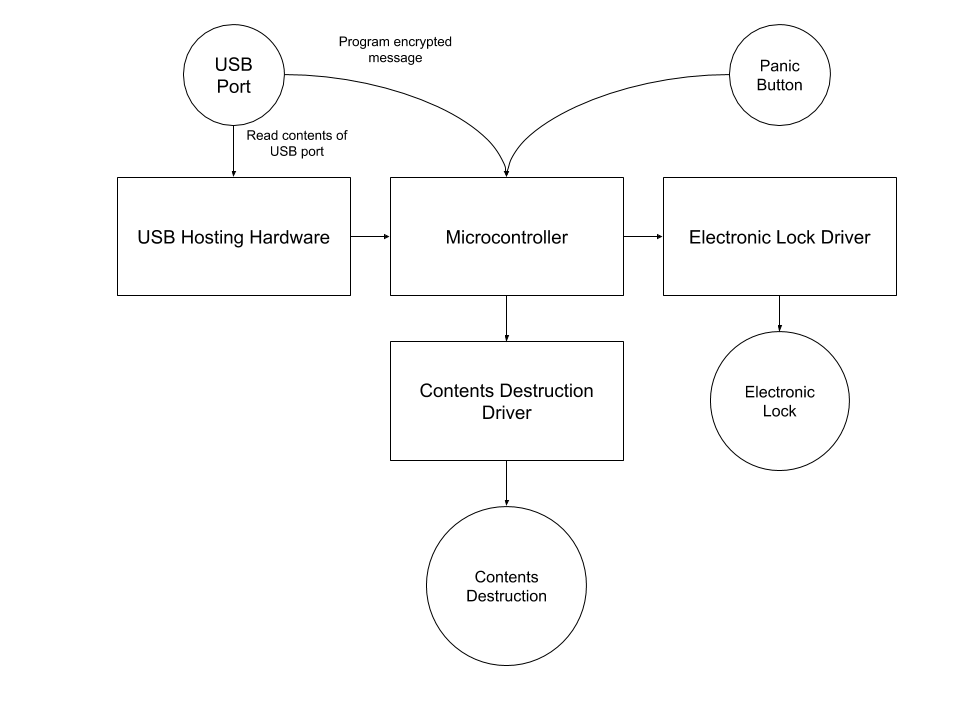
\includegraphics[scale=0.4]{briefcase_architecture_diagram.png}
    \caption{Briefcase Hardware Architecture}
    \label{fig:briefcase_architecture}
\end{figure}

As it is common for microcontrollers to not have USB hosting capabilities, USB hosting hardware is required to read the contents of a memory stick that is plugged into the concealed USB port. This hardware could be similar to the hardware found on the Arduino USB Host Shield \cite{arduinoUSBHost} As well as this, the concealed USB port must be connected to the chosen microcontroller in order to program the briefcase with the set encrypted message.

The microcontroller is connected to an electronic lock (such as a solenoid \cite{solenoidDigikey} or a motorised lock \cite{motorisedLock}). Microcontrollers are usually unable to drive such devices, so some form of hardware (such as a relay or a transistor) is anticipated. Furthermore, if the customer decides that they would like the contents of the briefcase destroyed in an emergency situation, a concealed panic button is connected to the microcontroller, which is also connected to a contents destruction mechanism via an appropriate driver. The contents destruction mechanism has not yet been formally decided and further research will be required to find an appropriate method. Potential methods include using hydraulics to spray ink onto the contents or installing a paper shredding mechanism within the briefcase. Each of these ideas have their own unique disadvantages, such as whether they make the briefcase safe for air travel or are too heavy to implement.

The microcontroller is also connected to a form of wireless communication, so it can communicate with the courier's handheld device during a transfer between couriers.

\begin{figure}[h]
    \centering
    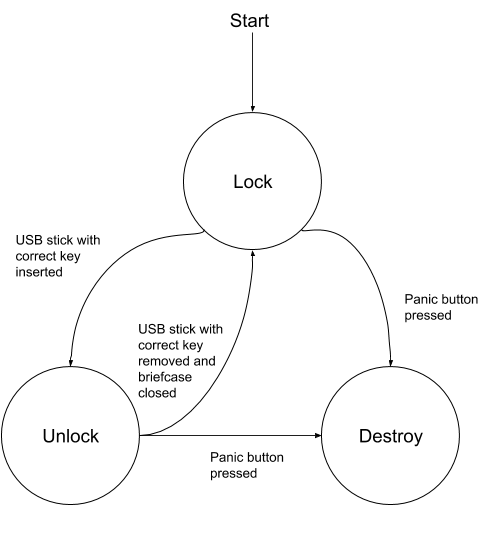
\includegraphics[scale=0.4]{briefcase_state_machine.png}
    \caption{Briefcase State Machine}
    \label{fig:briefcase_state_machine}
\end{figure}
The software architecture of the briefcase itself is simple and its behaviour can be described in the state machine in Fig. \ref{fig:briefcase_state_machine}. There are four states: \textit{Lock}, in which the briefcase is locked and the system is actively waiting for a USB memory stick to be inserted. If a USB memory stick is inserted, and contains the correct encrypted message, then the state machine moves to \textit{Unlock}, in which the briefcase is obviously unlocked. The system can only then move back to the \textit{Lock} state if the briefcase is closed and the USB stick containing the encrypted message is removed.

During a transfer of the briefcase between couriers, the succeeding courier must plug a USB stick containing their UID into the briefcase, this puts the system into the \textit{Transfer} state, in which the briefcase wirelessly communicates with the preceding courier's handheld device to signal that the transfer is approved and successful.

In all states, if this option is chosen by the customer, a transition to the \textit{Destroy} state can be made by pressing the  panic button. In this state, the contents destruction mechanism is activated. It is impossible to transition out of this state. Instead, it is intended that the platform will have to be manually be reprogrammed by one of our engineers. 